\chapter{Mustererkennung}

\paragraph{}
Unter dem Begriff Mustererkennung versteht man die auomatische Verarbeitung und
Auswertung von Mustern und deren Zuordnung zu vorbestimmten Klassen. Die Muster%
erkennung setzt eine problemangepa\ss{}te Me\ss{}weterfassung voraus. Bild
\ref{fig:mustererkennung} zeigt die Struktur eines akustischen
Mustererkennungssytems.

\begin{figure}[ht]
\centering
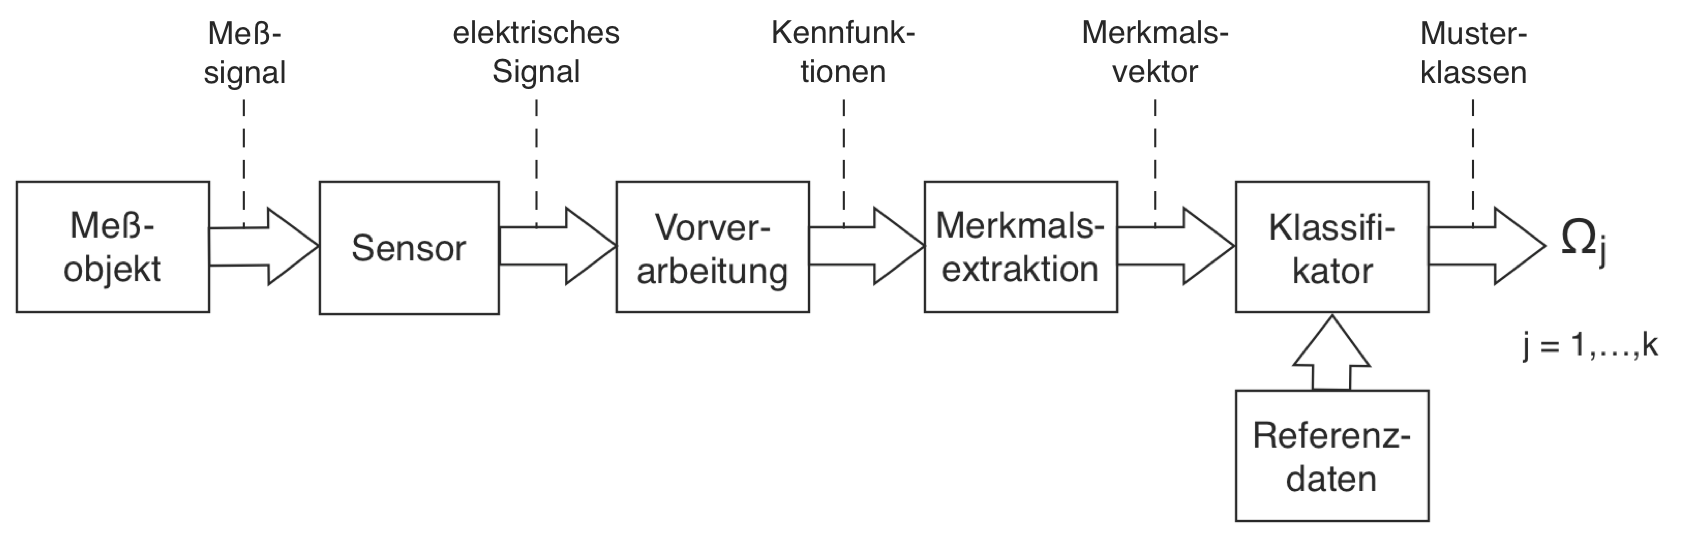
\includegraphics[width=1\textwidth]{mustererkennung}
\caption{Struktur der Mustererkennung}
\label{fig:mustererkennung}
\end{figure}

\paragraph{}
Das \textbf{Me\ss{}objekt} ist der zu erkennende Gegenstand. In der 
Ger\"auschdiagnose werden Me\"objekte nach einem bestimmten akustischen
Verhalten untersucht.

\paragraph{}
Der \textbf{Sensor} (Me\ss{}wertaufnehmer) wandelt die vom Me\ss{}objekt
ausgestrahlten mechanischen oder akustischen Schwingungen (Me\ss{}signale) in
elektrische Signale um. Wegen ihrer Unempfindlichkeit gegen\"uber
Umgebungsger\"auschen werden bevorzugt K\"orperschallaufnehmer f\"ur die
Me\ss{}werterfassung eingesetzt.

\paragraph{}
Durch die \textbf{Vorverarbeitung} wird ein Signal in eine f\"ur die weitere
Verarbeitung geeignetere Form gebracht. Sie beinhaltet im wesentlichen die
AD-Wandlung des analogen elektrischen Signals und die Transformation in
geeignete Kennfunktionen. Dabei mu\ss{} eine optimale Aussteuerung des
AD-Wandlers gew\"ahrleistet sein. Dementsprechend m\"ussen Verst\"arkungs-
bzw. D\"ampfungsma\ss{}nahmen durchgef\"uhrt werden. Au\ss{}erdem sind die
Bedingungen des Abtasttheorems zu erf\"ullen, was gegebenenfalls den Einsatz
eines Antialiasing-Filters erfoldert.

\paragraph{}
Auf der Stufe der \textbf{Merkmalsextraktion} werden aus den Kennfunktionen
zun\"achst Kennwerte ermittelt, die Beitr\"age zur Klassentrennung liefern
k\"onnen. Um den Merkmalen Chancengleichheit bez\"uglich der Klassentrennung
einzur\"aumen, erfolgt h\"aufig eine Kennwertnormierung (z.B. in den Werte%
bereich [0..1]). Eine weitere Hauptaufgabe der Merkmalsextraktion ist die
Auswahl der signifikantesten Merkmale hinsichtlich ihrer Klassentrennungs%
f\"ahigkeit, die eine Merkmalsselektion bedeutet. Mit der Auswahl der Merkmale
ist eine Datenreduktion (Merkmalsreduktion) verbunden. Zus\"atzlich kann eine
Merkmalsreduktion liefert schlie\ss{}lich Merkmalsvektoren, die als Komponenten
die verschiedenen Merkmale bzw. deren Transformation enthalten.

\paragraph{}
Der Merkmalsvektor wird dem \textbf{Klassifikator} zur Verf\"ugung gestellt.
Dieser allein ist f\"ur eine Klassifikation nicht ausreichend. Ein Muster%
erkennungssystem kann eine Erkennungsaufgabe nur dann automatisch l\"osen,
wenn es bestimmte Informationen \"uber das zu erkennende Objekt und die zu
differenzierenden Klassen besitzt. Der Klassifikator ben\"otigt also f\"ur die
Zuordnung des Me\ss{}objektes zu einer Lernphase zu berechnen sind. Die Art der
klassenspezifischen Information h\"angt vom verwendeten Klassifikatortyp ab. Je
nach Art der Entscheidungsfunktion kann es sich dabei um eine Stichprobe
vorklassifizierter Muster oder um Klassenrepr\"asentanten (Parameter) handeln,
die aus der Lernstichprobe berechnet werden. Falls keine Klassifikation eines
Me\ss{}objektes mit bestimmter Wahrscheinlichkeit m\"oglich ist, kann eine
R\"uckweisung erfolgen.\\
Um ein Urteil \"uber die Lernstichprobe zu bilden und die Eignung eines
Klassifikators f\"ur diese zu testen, wird die Lernstichprobe klassifiziert.
Dir Klassifikation der Lernmuster selbst, also der Proze\ss{} der Re%
klassifikation, liefert eine scheinbare Fehlerrate. Im Idealfall sollte
diese 0\% betragen. Diese sogenannte Reklassifikationsfehlerrate wird als
Akzeptanzma\ss{} daf\"ur angesehen, ob eine Lernstichprobe f\"ur die
Klassifikation unabh\"angiger Objekte geeignet ist.\\
Die Reklassifikationsfehlerrate ist nicht allein ausreichend, um die Leistung
der Mustererkennung mit dem gew\"ahlten Klassifikator zu beurteilen. Praktisch
geht man so vor, eine unabh\"angige Teststichprobe mit bekannter Klassen%
zugeh\"origkeit der Objekte neu zu klassifizieren. Dieser Vorgang wird \textbf{%
Testklassifikation} genannt. Die Fehlerrate der Testklassifikation ist ein
reales Fehlerma\ss{} f\"ur den eingesetzten Klassifikator und liegt in der Regel
h\"oher als die scheinbare Fehlerrate bei Reklassifikation. Damit l\"a\ss{}t
sich die Wirksamkeit eines Erkennungssystem beurteilen.

\begin{figure}[ht]
\centering
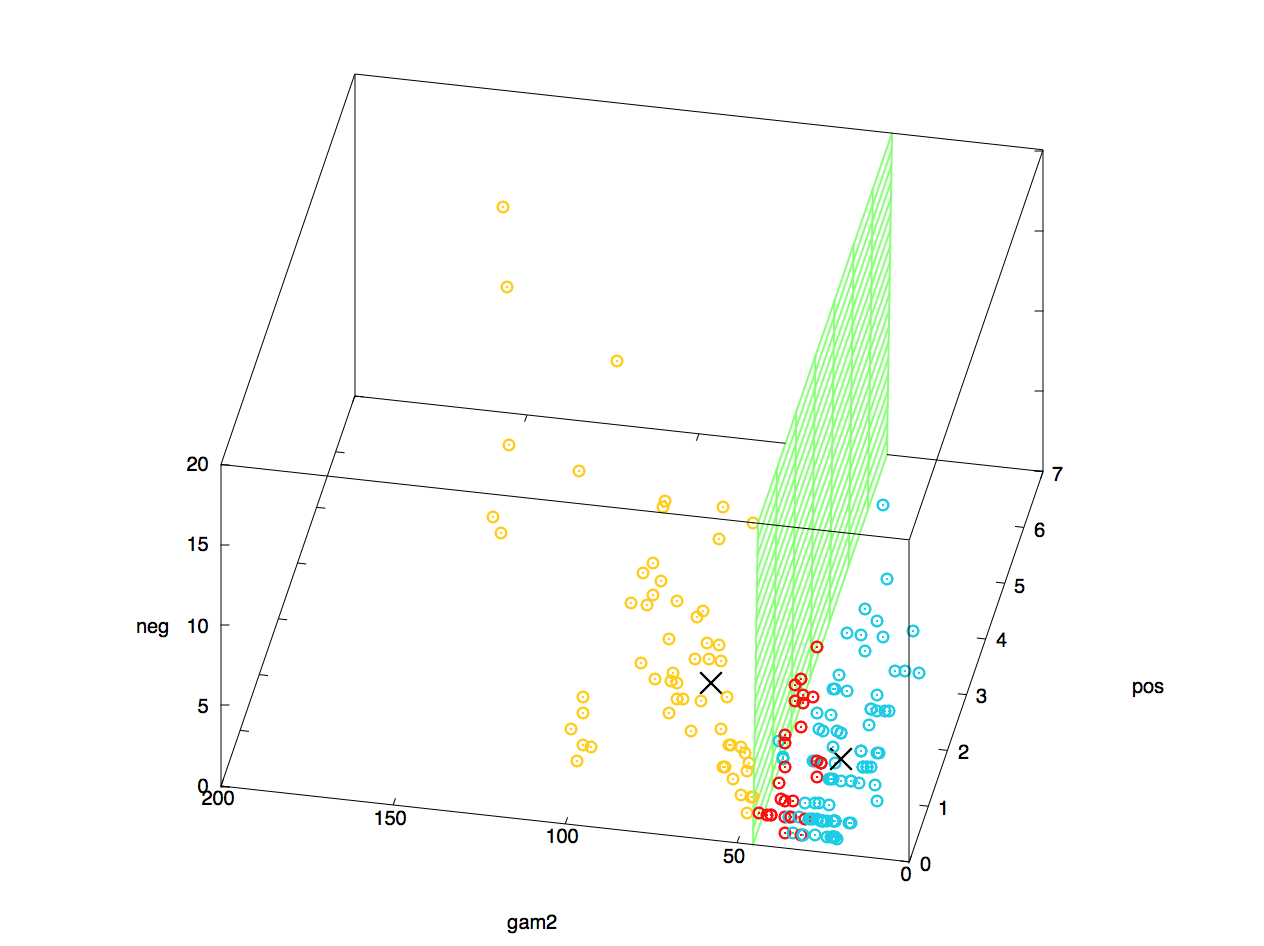
\includegraphics[width=1\textwidth]{mindestabstandEuklid}
\caption{Ergebnis der Pr\"ufung des Mindestabstand Klassifikators (Euklidischer
Abstand)}
\end{figure}

\begin{figure}[ht]
\centering
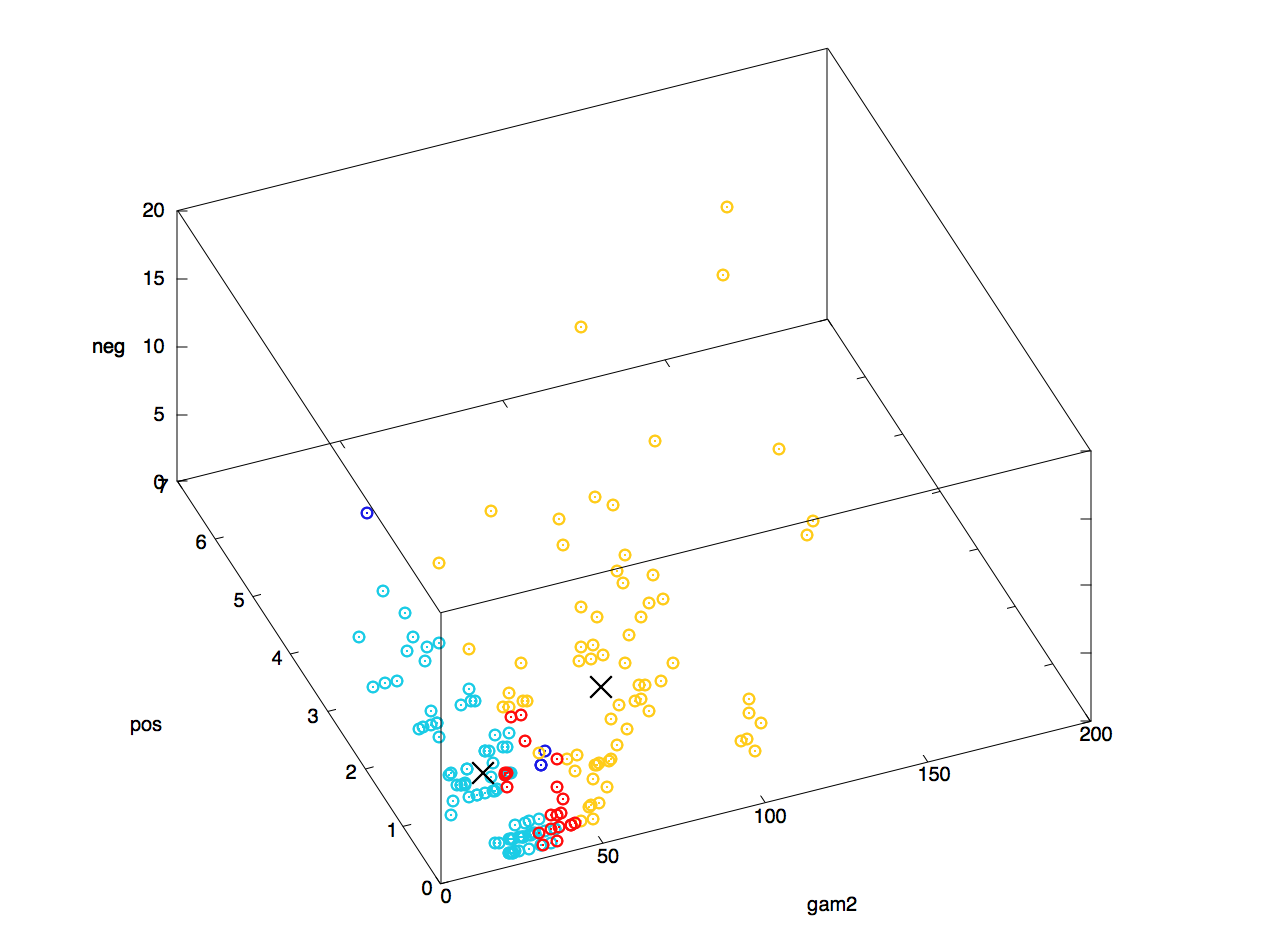
\includegraphics[width=1\textwidth]{mindestabstandMahalanobis}
\caption{Ergebnis der Pr\"ufung des Mindestabstand Klassifikators (Mahalanobis-%
Distanz)}
\end{figure}

\begin{figure}[ht]
\centering
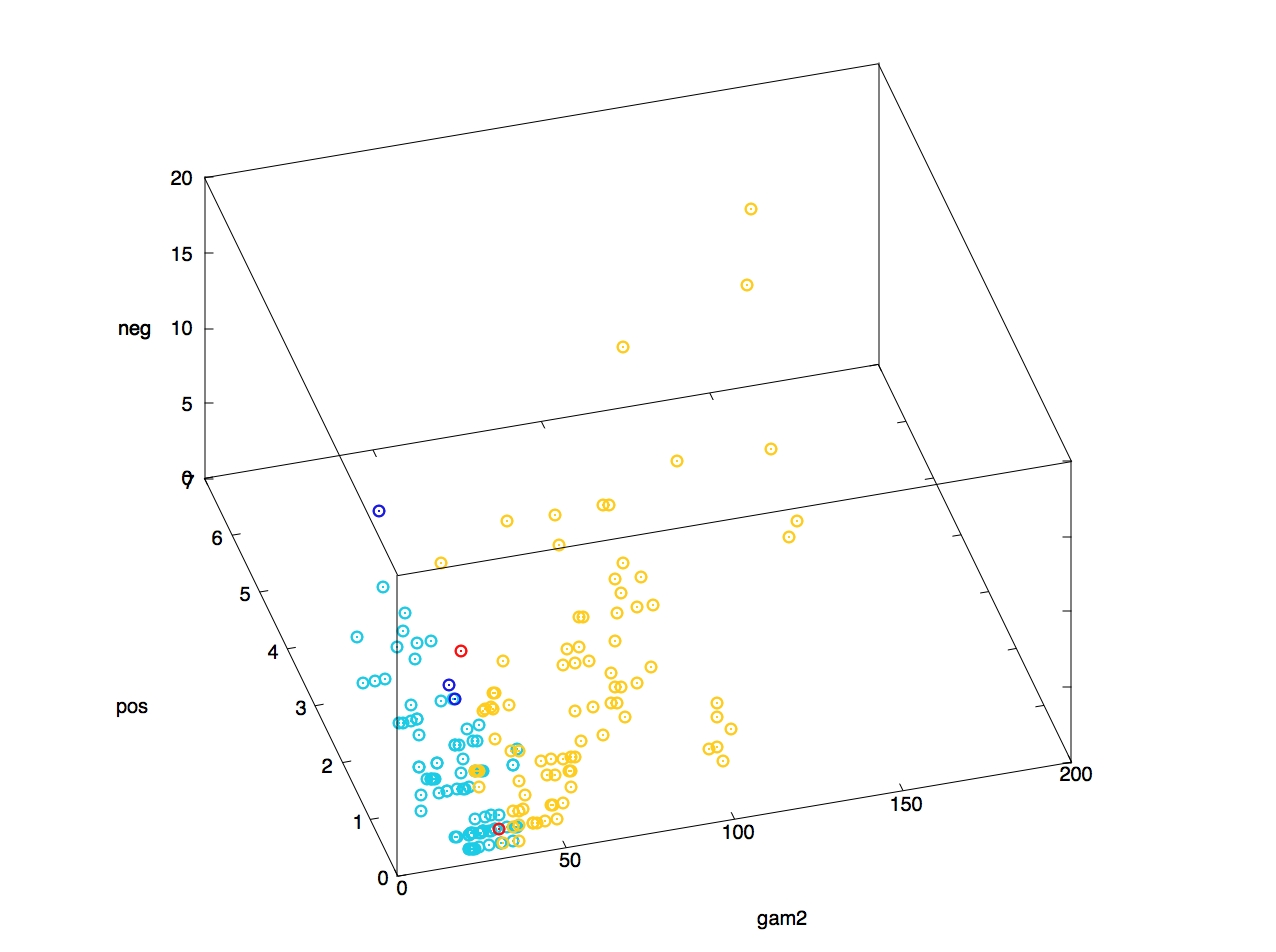
\includegraphics[width=1\textwidth]{naiverBayes}
\caption{Ergebnis der Pr\"ufung des naiven Bayes-Klassifikators}
\end{figure}

\begin{figure}[ht]
\centering
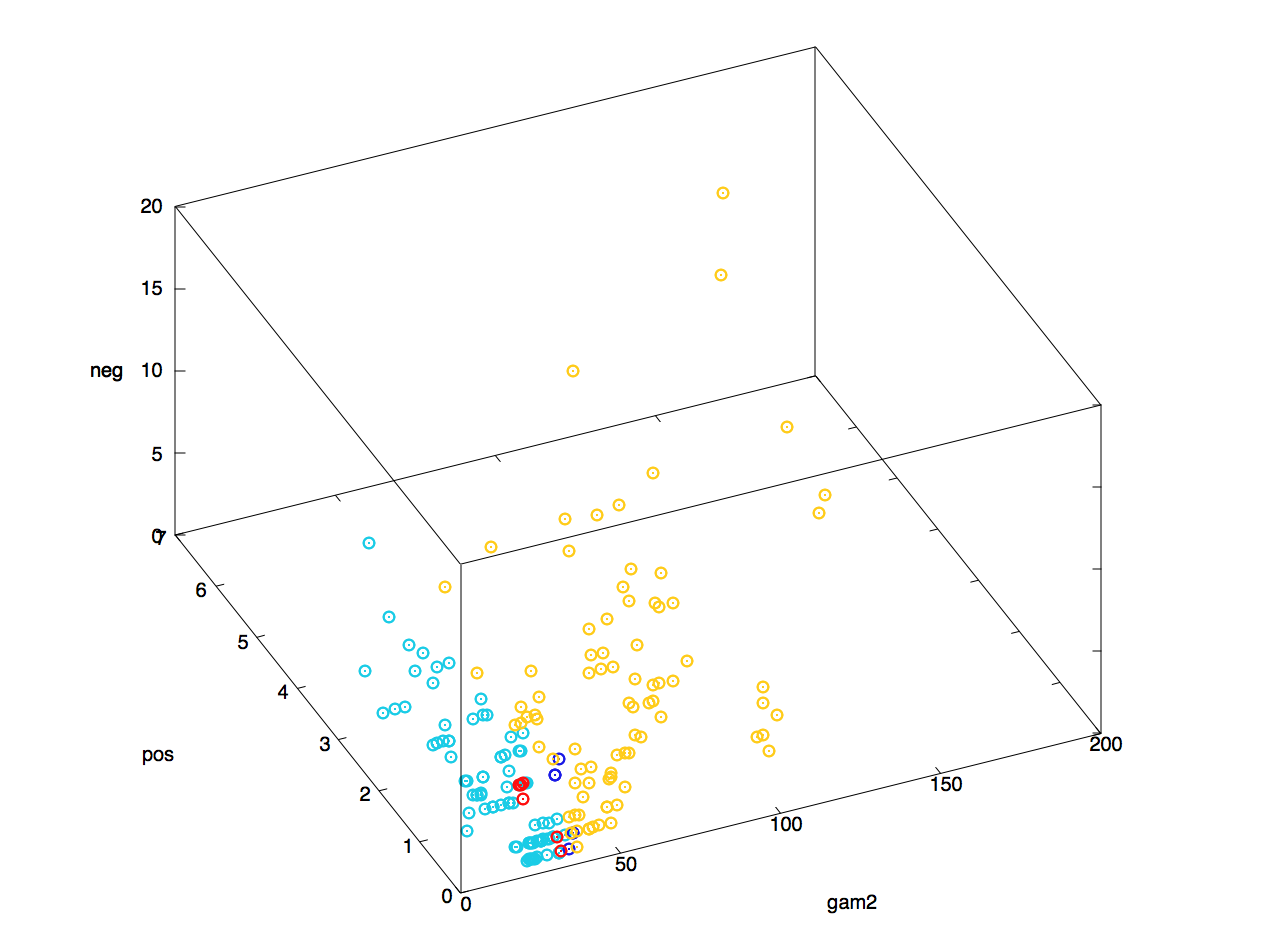
\includegraphics[width=1\textwidth]{neuronalesNetz}
\caption{Ergebnis der Pr\"ufung des neuronalen Netzes}
\end{figure}